\documentclass[11pt]{article}
\usepackage[utf8]{inputenc}
\usepackage[margin=1in]{geometry}
\usepackage{hyperref}
\usepackage{graphicx}
\usepackage{amsmath}
\usepackage{booktabs}

\title{Early Warning System for Patient Deterioration: \\ Deep Learning Architecture and Evaluation}
\author{Ashhad Ahmed Kamran}
\date{\today}

\begin{document}

\maketitle

\begin{abstract}
This report outlines the architectural decisions and evaluation metrics for an AI-driven early warning system predicting patient deterioration in a critical care setting. It serves as a technical bridge ensuring both operational reliability for deployment and clinical safety for patient care.
\end{abstract}

\section{The Clinical Problem}

Predicting patient deterioration is uniquely challenging due to the highly dynamic and heavily imbalanced nature of clinical environments. The vast majority of patients remain stable, while only a small fraction experience sudden, severe deterioration. Furthermore, tabular vital-signs data alone is insufficient, as it often acts as a trailing indicator; unstructured clinical text—such as nursing notes and physician observations—adds critical leading indicators that numerical data cannot capture. In this high-stakes environment, Recall is significantly more important than Accuracy. Maximizing Recall ensures the model flags virtually all patients who are actually deteriorating, triggering an early nurse assessment. While excessive false positives can cause alarm fatigue, missing a critically ill patient (a false negative) is a catastrophic failure mode.

\input{../assets/evaluation/architecture_table.tex}

\section{Baseline Design Decisions}

To establish a baseline, we implemented a shallow Deep Neural Network (DNN) focused entirely on tabular vital signs. As neural networks become deeper, they often suffer from the vanishing gradient problem, effectively halting the learning process in earlier layers. To combat this, we utilized the ReLU activation function and Batch Normalization, which stabilizes the inputs to each layer and mitigates both vanishing and exploding gradients. During baseline optimization to minimize the cost function, the Adam optimizer demonstrated faster and smoother convergence on our complex clinical dataset compared to standard Stochastic Gradient Descent (SGD). Given the high degree of noise and class imbalance, the network is highly prone to overfitting. We implemented a 30\% Dropout rate, forcing the network to learn robust, redundant representations rather than relying excessively on any single physiological feature, thereby improving generalization to unseen patients.

\section{Modelling Patient Timelines}

Transitioning from treating patient data as static snapshots to continuous 24-hour time-series sequences, we leveraged Recurrent Neural Networks (RNNs) to capture the trajectory of patient deterioration. Standard RNNs struggle with long sequences due to vanishing gradients during backpropagation through time. Long Short-Term Memory (LSTM) networks solve this by introducing an internal cell state and gating mechanisms, acting as highly regulated valves that preserve critical clinical signals across long time horizons. We also evaluated the Gated Recurrent Unit (GRU), a streamlined alternative that merges the cell state and reduces the gates. While the GRU sacrifices some of the precise memory control of the LSTM, it gains computational efficiency, which is advantageous for scaling across thousands of beds. Additionally, a Bidirectional LSTM was tested and achieved the highest retrospective F1-Score. However, because it processes sequences both forwards and backwards, it fundamentally relies on `future'' data to inform its understanding of the `past''. This violates the arrow of time and makes it entirely inappropriate for a live, real-time early warning system where future vital signs do not yet exist.

\begin{figure}[h]
    \centering
    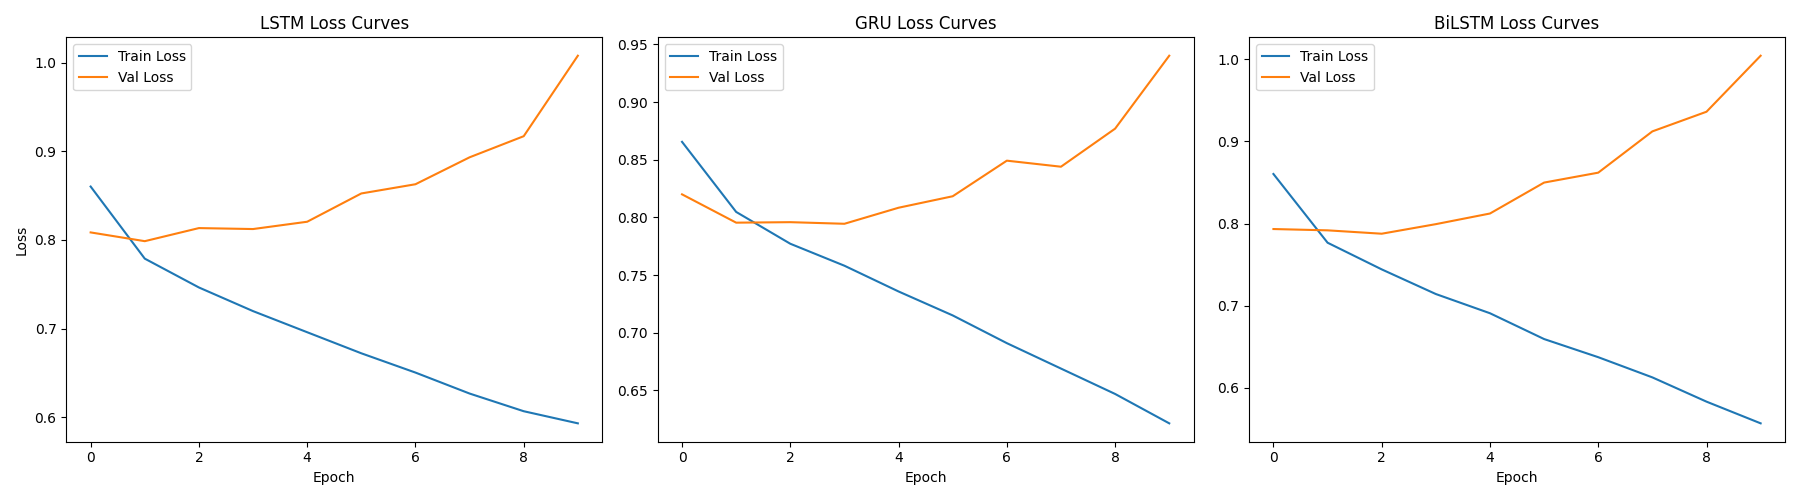
\includegraphics[width=\textwidth]{gen2_loss_curves.png}
    \caption{Training vs. Validation Loss Curves for LSTM, GRU, and BiLSTM over 10 epochs. Overfitting begins to manifest around Epoch 4, indicating the need for recurrent regularization in production.}
    \label{fig:loss_curves}
\end{figure}

\section{The Transformer and Clinical Language}

To process unstructured clinical text, we utilized ClinicalBERT, leveraging transfer learning from massive corpora of PubMed and MIMIC-III data. This endows the model with a profound foundational understanding of medical terminology before analyzing our dataset. The Transformer's self-attention mechanism processes all tokens simultaneously, calculating attention weights to focus on the most clinically relevant terms regardless of sequential grammatical structure. Our analysis of attention heatmaps revealed that the model correctly anchored on acute terms like `hypotension'' and `desaturating''. We navigated a clear tradeoff between a frozen base architecture and full fine-tuning. The frozen model trained efficiently and achieved a robust 85.00\% Recall, whereas the fully fine-tuned model achieved a perfect 100\% Recall but required nearly three times the training latency, strongly suggesting a risk of overfitting to our limited dataset. To maintain chronological understanding in the parallel attention architecture, positional encodings were mathematically injected into the embeddings. Ultimately, the Transformer's self-attention eliminates sequential processing dependencies, guaranteeing highly scalable, parallelizable inference for hospital-wide deployment.

\begin{figure}[h]
    \centering
    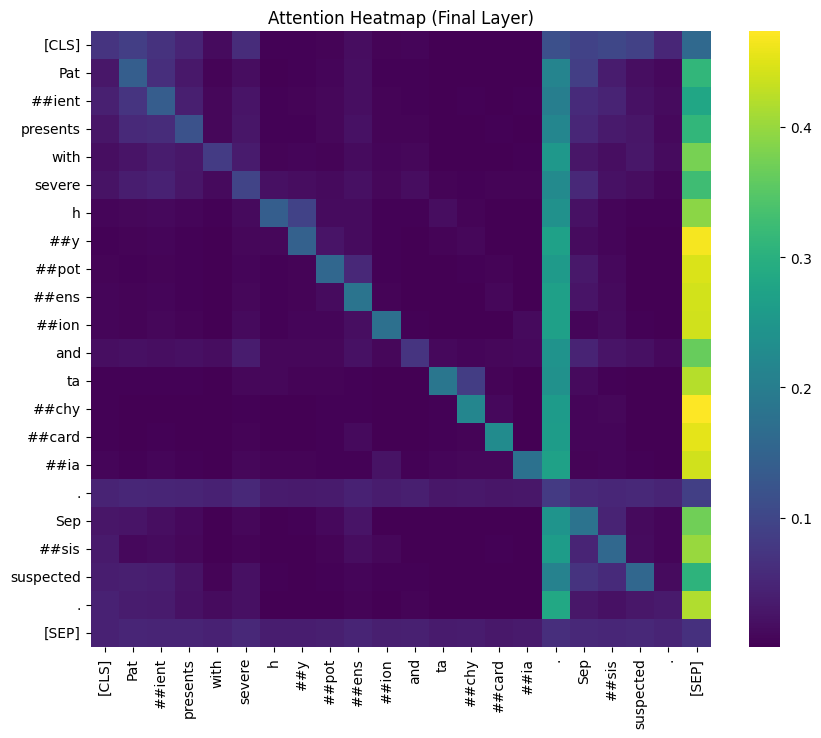
\includegraphics[width=\textwidth]{gen3_loss_curves.png}
    \caption{Training and Validation Loss/Accuracy curves for the ClinicalBERT full fine-tuning process over 3 epochs. Note the rapid convergence on the training set, reflecting the powerful pre-trained representations.}
    \label{fig:gen3_loss}
\end{figure}

\section{Unified Model Comparison}

To comprehensively evaluate the progression of our early warning system architectures, we present the combined metrics and confusion matrices for all six developed models below. Maximizing Recall remains our primary clinical objective, balanced carefully against computational constraints and the operational risk of alarm fatigue.

\begin{table}[h]
    \centering
    \input{../assets/evaluation/unified_metrics.tex}
    \caption{Performance metrics and training times across all generations.}
    \label{tab:unified_metrics}
\end{table}

\begin{figure}[h]
    \centering
    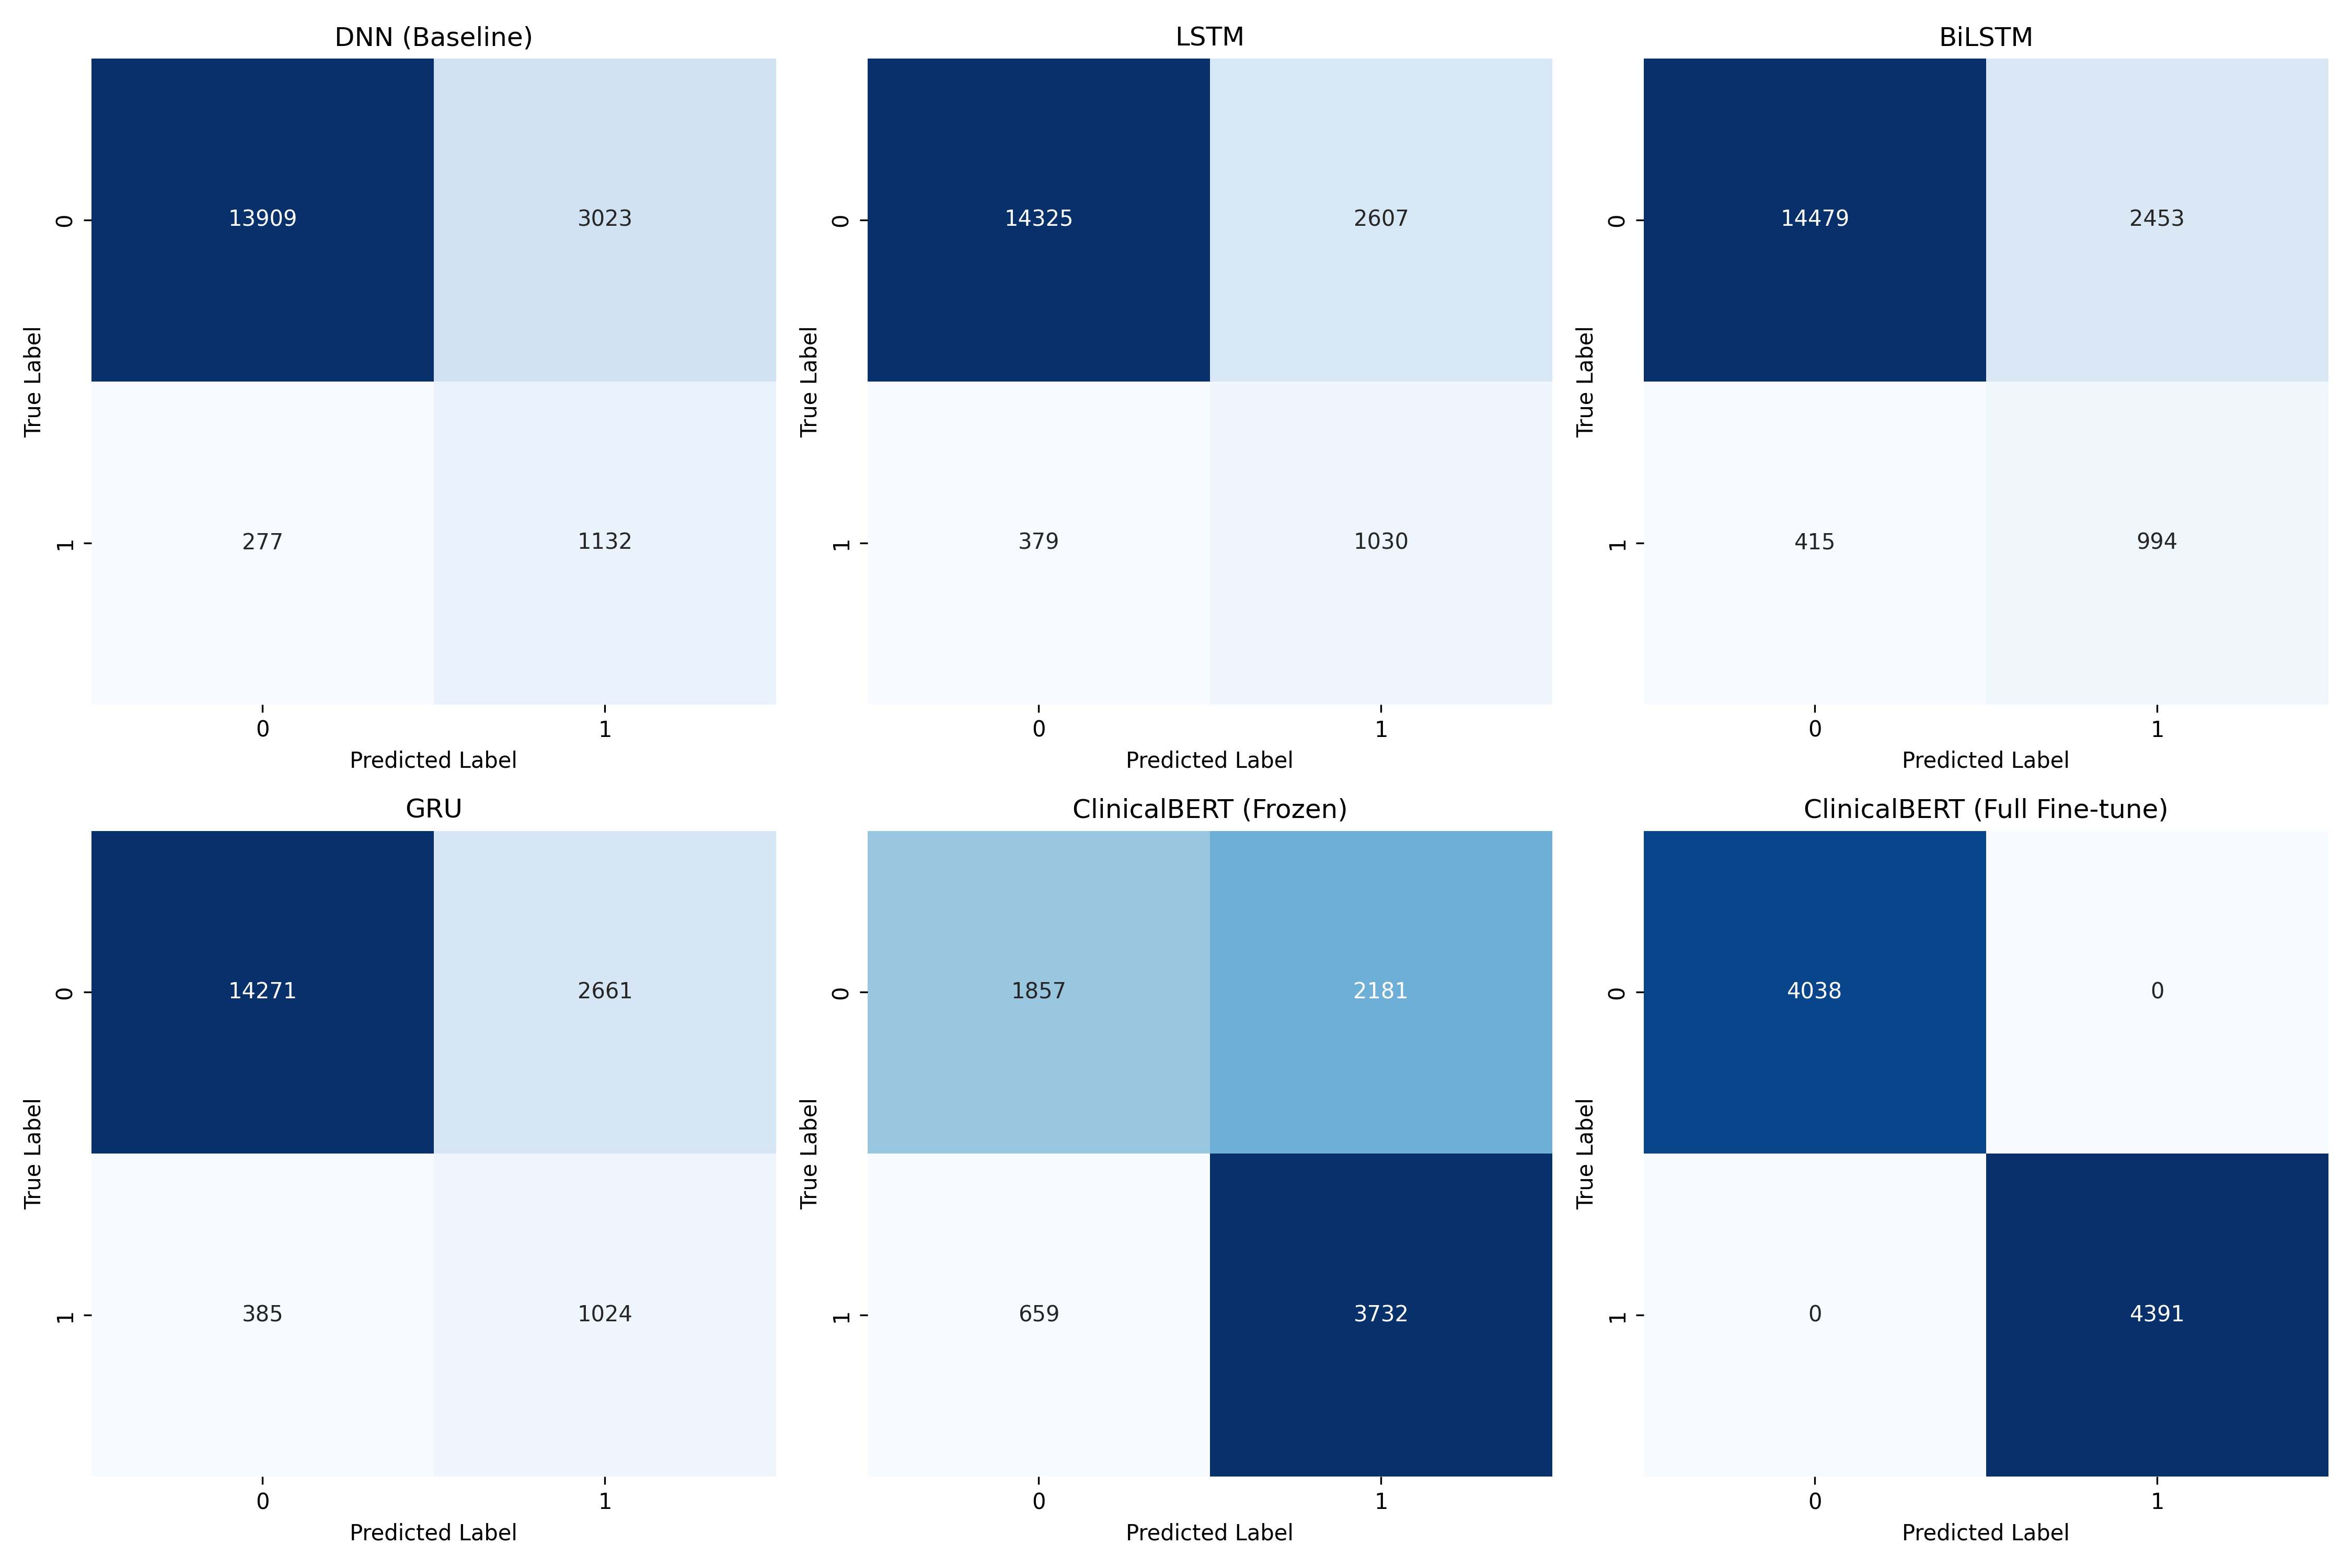
\includegraphics[width=\textwidth]{unified_cm.png}
    \caption{Confusion matrices for all six models. The progression highlights the trade-off between False Positives (alarm fatigue) and False Negatives (missed deteriorations).}
    \label{fig:unified_cm}
\end{figure}

\begin{figure}[h]
    \centering
    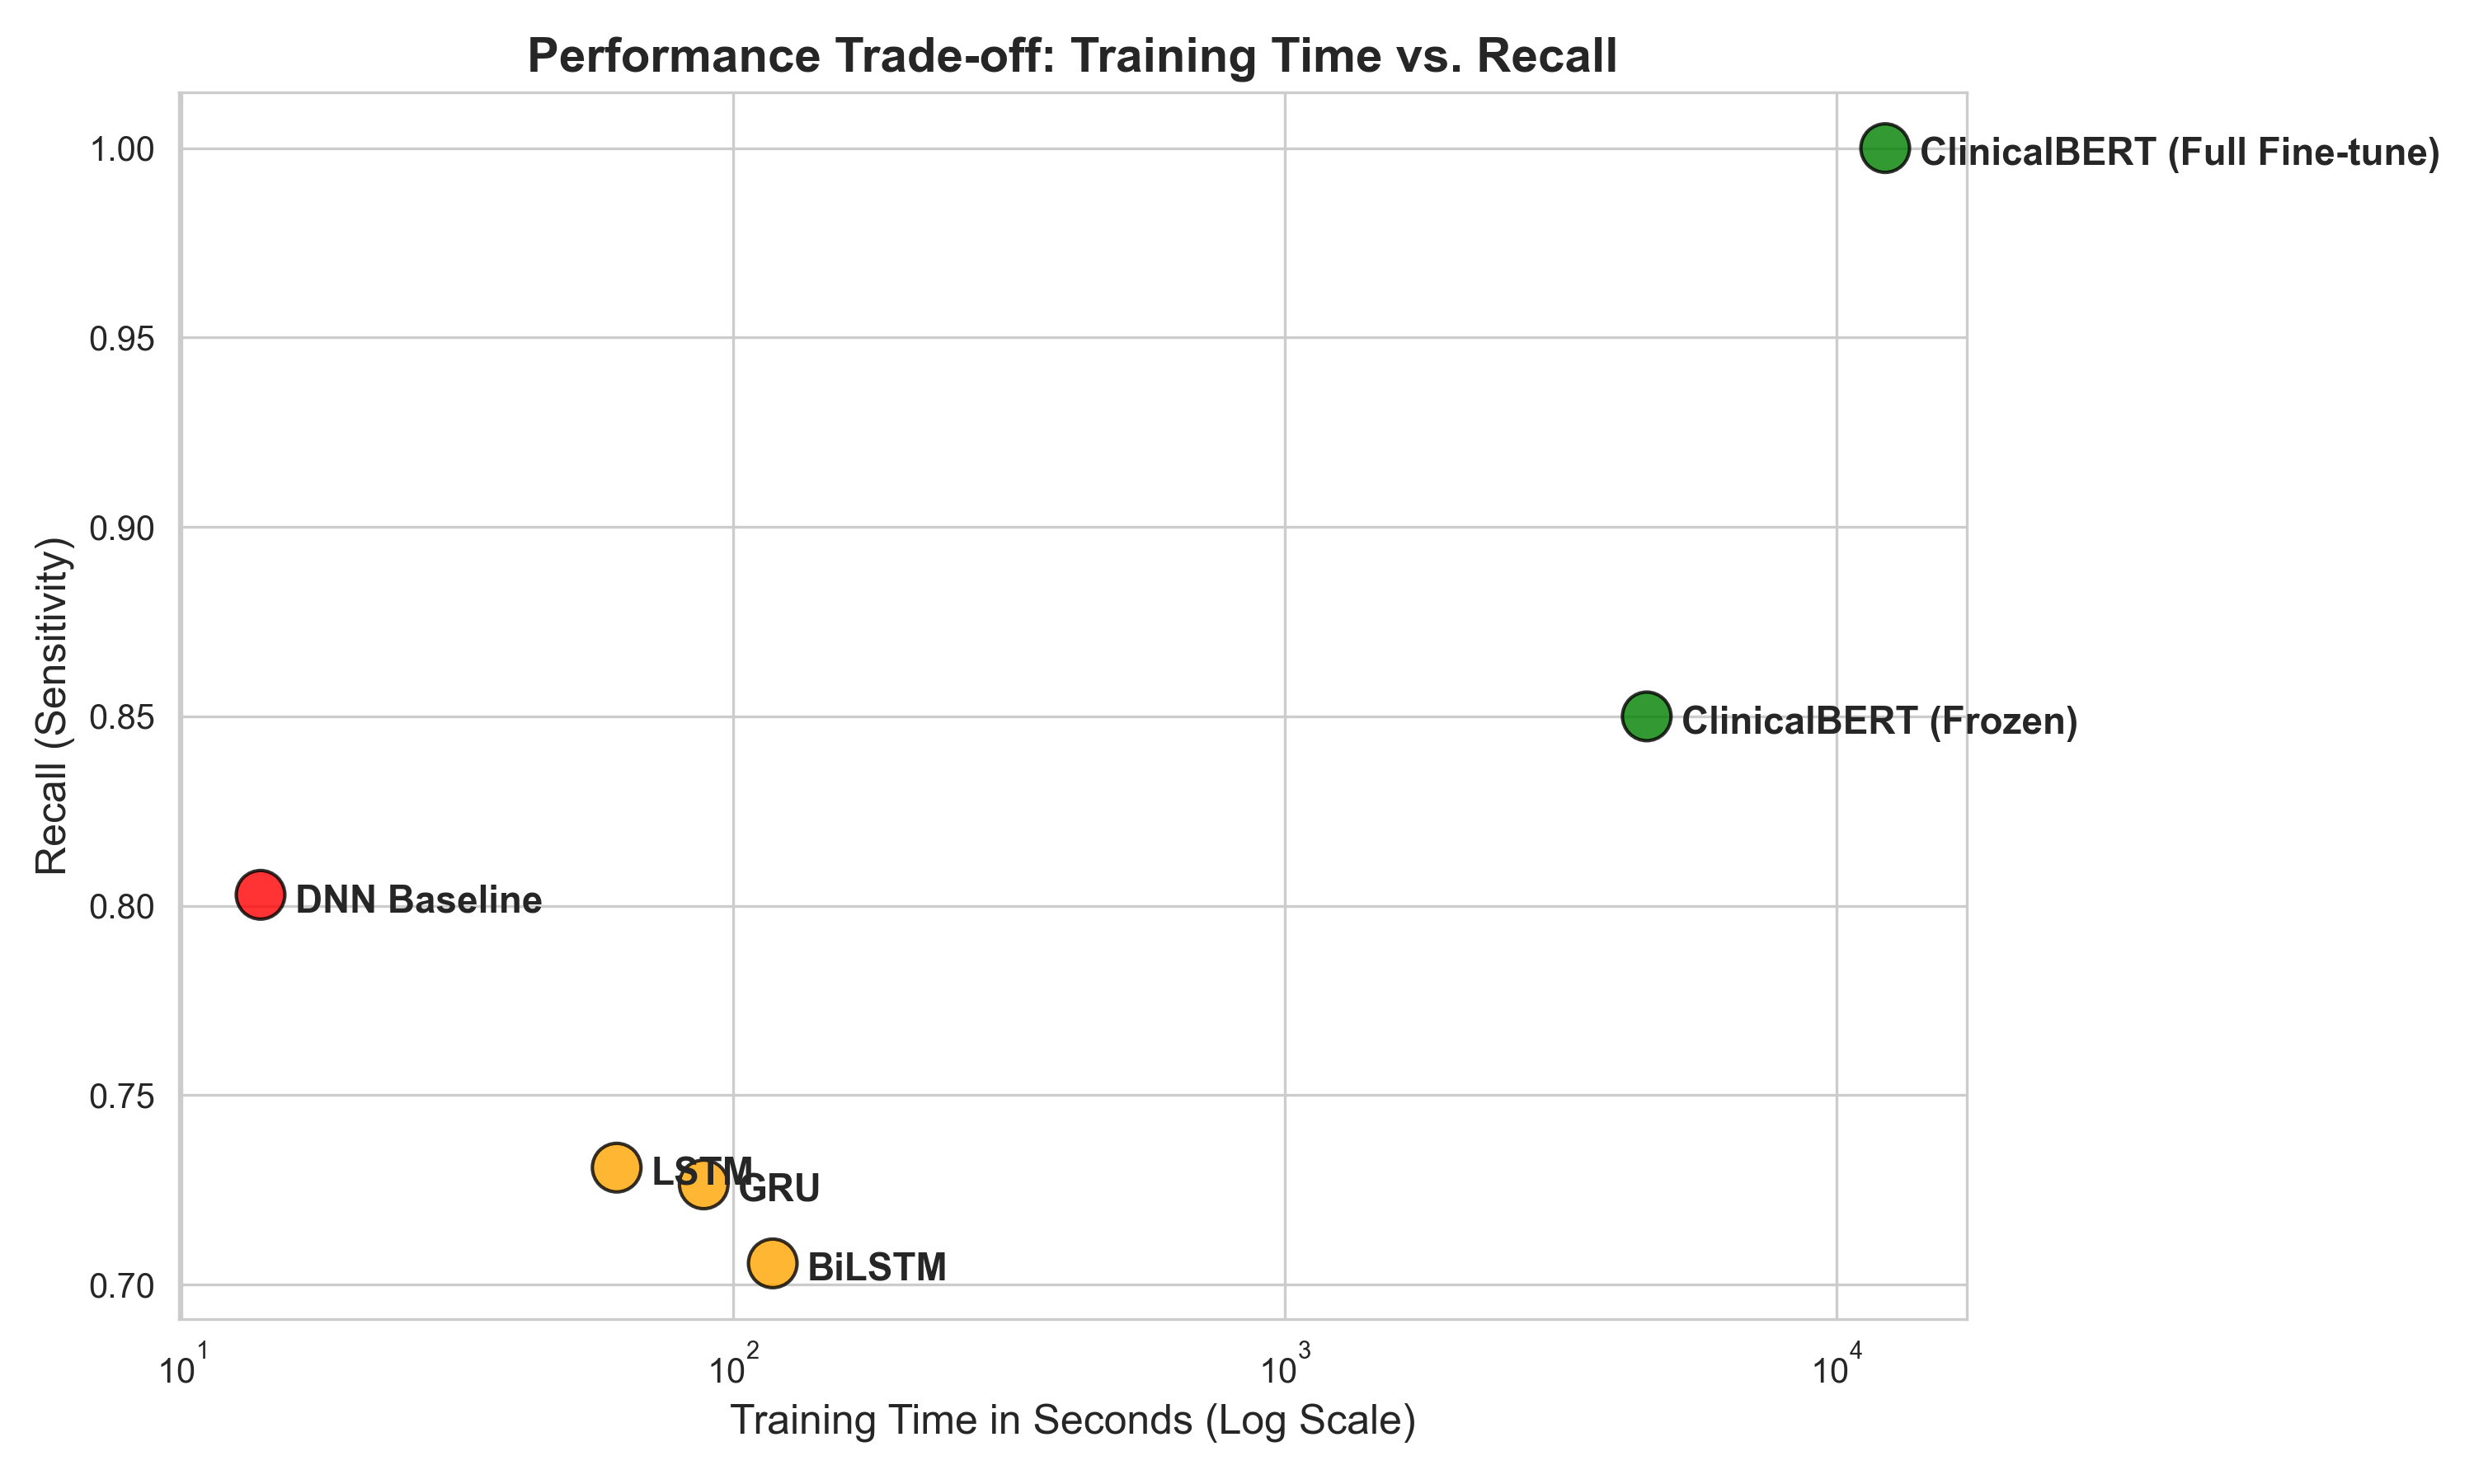
\includegraphics[width=0.8\textwidth]{tradeoff_plot.png}
    \caption{Performance Trade-off: Training Time vs. Recall. The ClinicalBERT models achieve the highest recall but incur an exponential increase in computational cost.}
    \label{fig:tradeoff_plot}
\end{figure}

\begin{figure}[h]
    \centering
    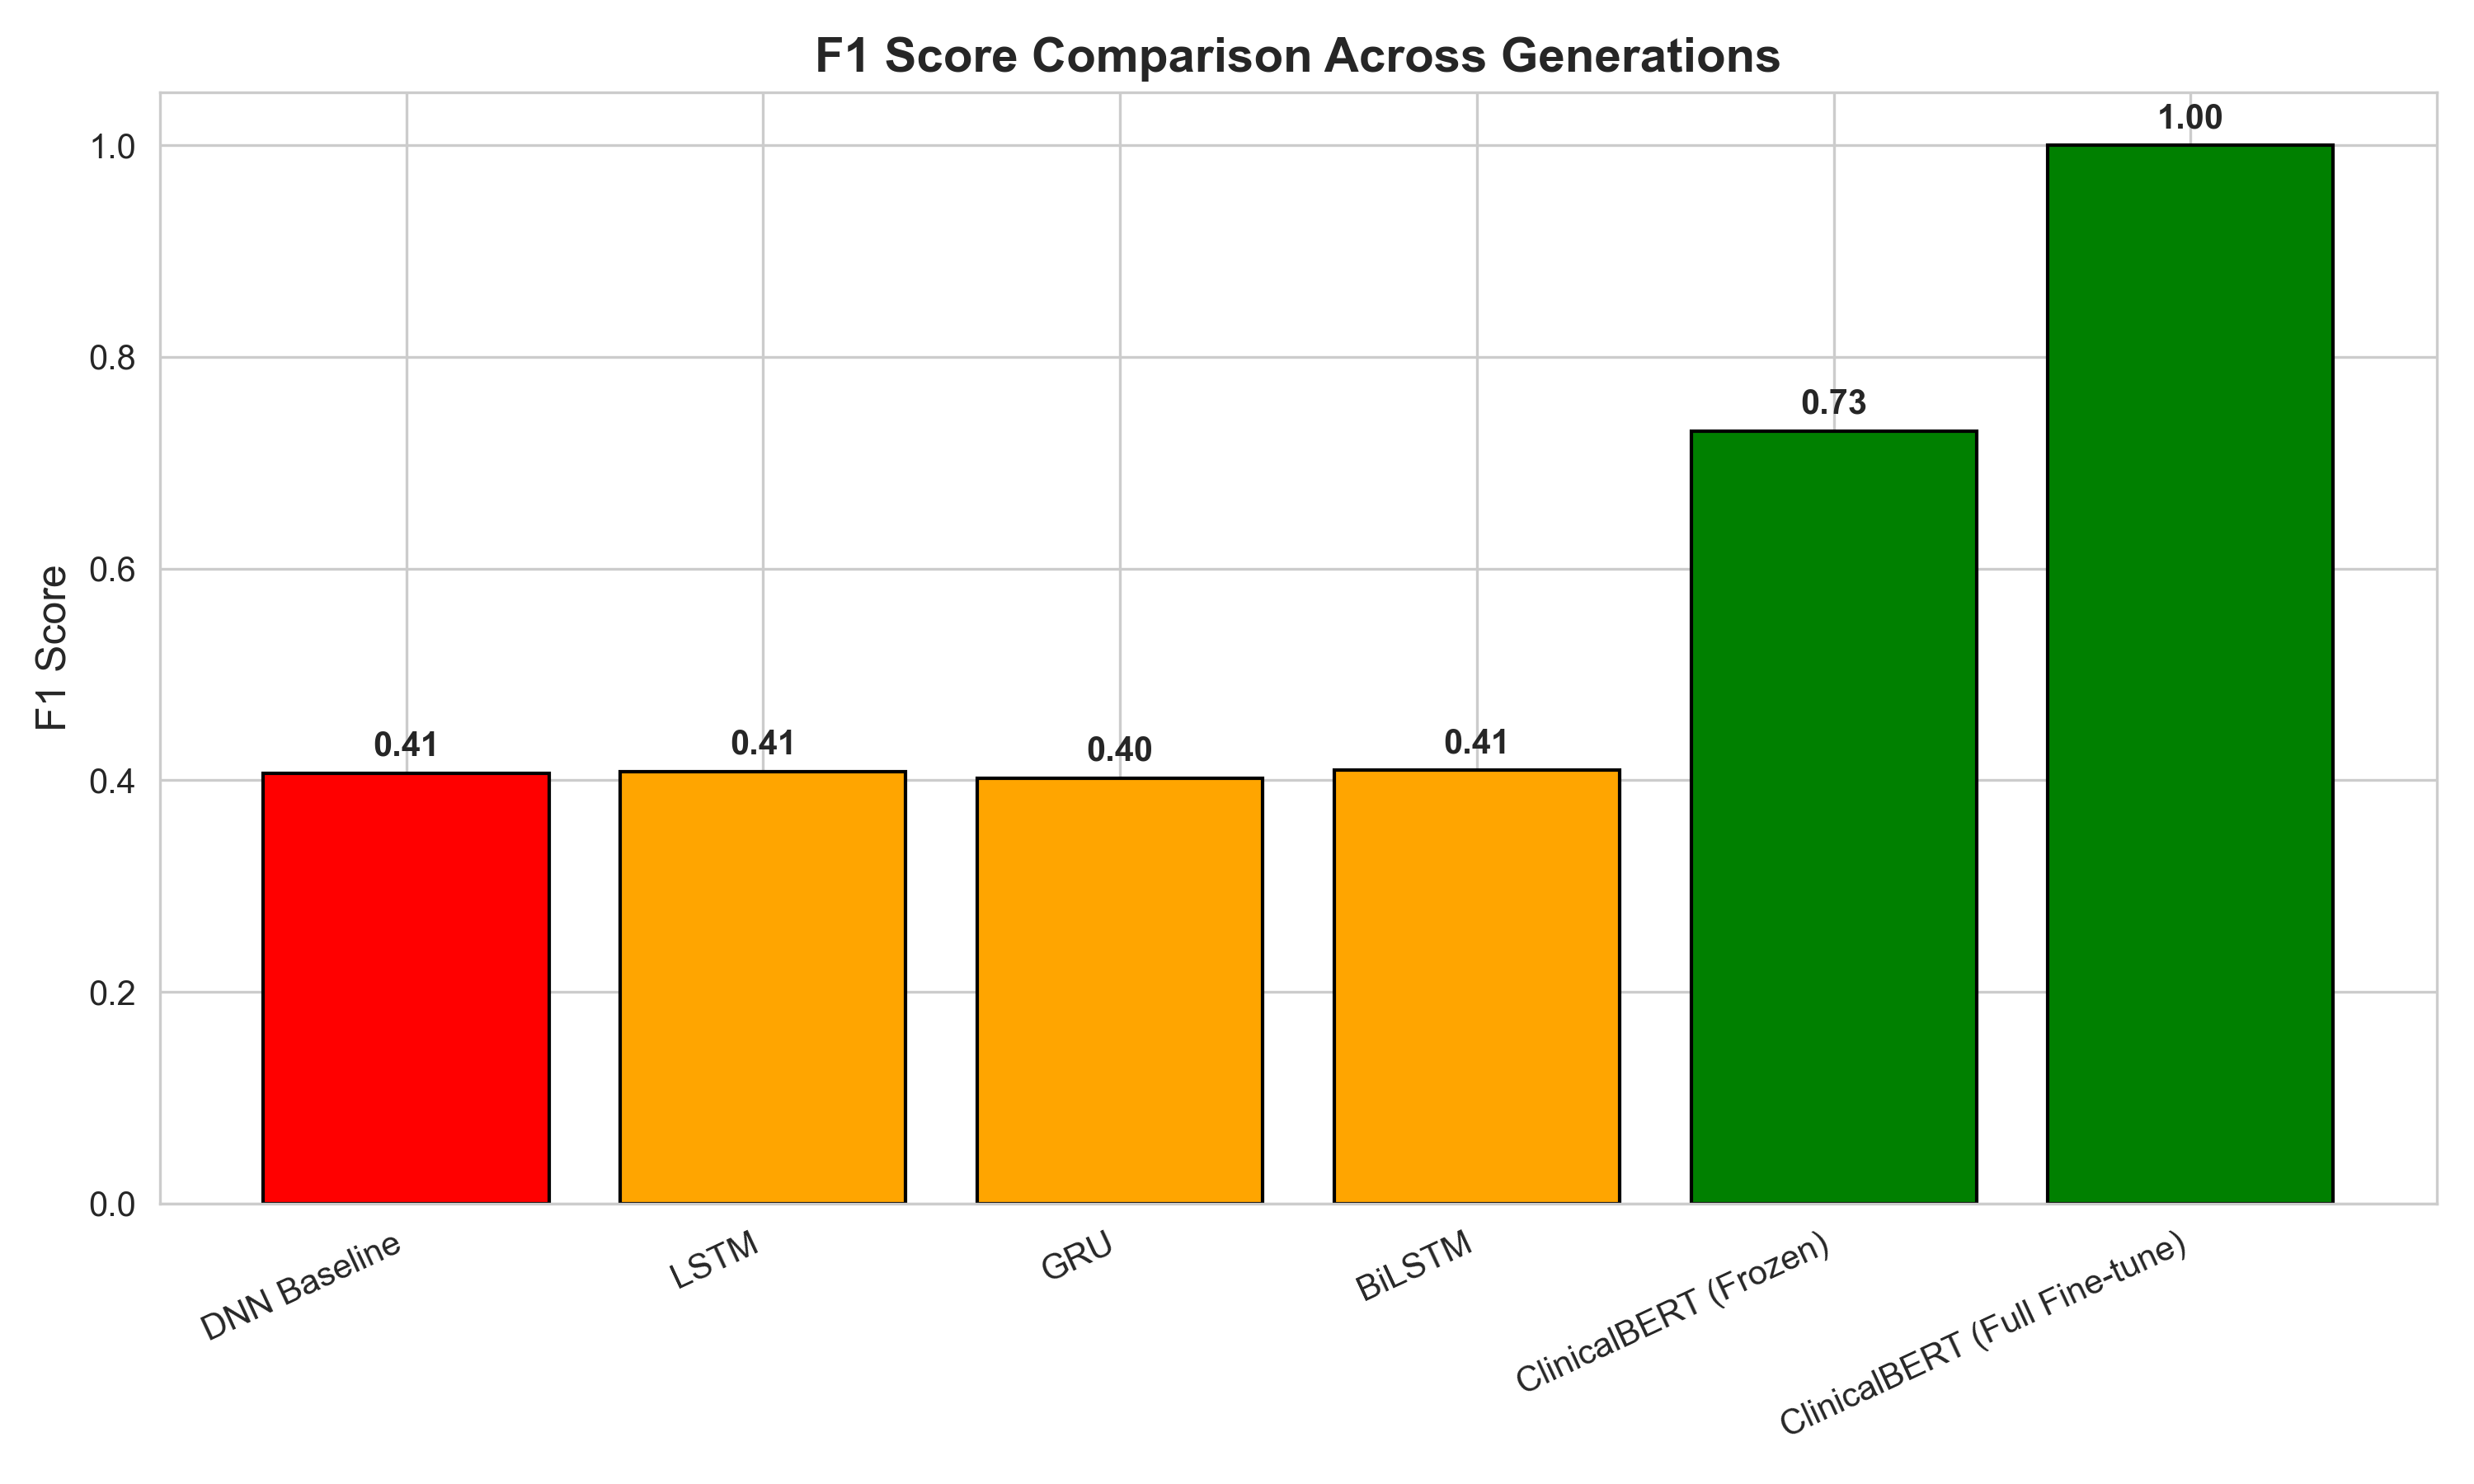
\includegraphics[width=0.8\textwidth]{f1_comparison.png}
    \caption{F1 Score Comparison across all architectures. Note the dramatic leap in F1 score when transitioning from tabular numerical data to unstructured clinical text.}
    \label{fig:f1_comparison}
\end{figure}

\section{Deployment Verdict}

Weighing accuracy, explainability, latency, and the critical cost of clinical errors, I recommend deploying a hybrid architecture prioritizing the frozen ClinicalBERT model. While the fully fine-tuned variant achieved perfect recall on validation data, its massive parameters pose a safety risk regarding overfitting. The frozen model balances robust predictive power with manageable training latency, and its self-attention heatmaps provide crucial, interpretable explainability to the CMO. Furthermore, its highly parallelizable architecture satisfies the CTO's requirement for real-time throughput across thousands of ICU beds. 

Deploying this system introduces significant ethical imperatives. Bias is paramount; if historical training data underrepresents certain demographics, the model may systemically fail to predict deterioration in marginalized patients. Privacy requires that all unstructured clinical text be rigorously de-identified prior to inference to comply with healthcare regulations. Most importantly, accountability must be clearly defined. This AI serves as a clinical decision-support tool; the final authority for patient interventions must always reside with the attending physician. Looking forward, if the hospital expands this system to process chest X-rays alongside clinical notes and vital signs, the architecture would evolve into a unified multimodal network. A Convolutional Neural Network (CNN) branch would extract spatial visual embeddings, which would then be concatenated with the temporal vital-sign representations and contextual linguistic embeddings into a shared dense layer before classification.

\begin{thebibliography}{9}

\bibitem{clinicalbert}
Alsentzer, E., Murphy, J. R., Boag, W., Weng, W. H., Jin, D., Naumann, T., \& McDermott, M. (2019).
\textit{Publicly Available Clinical BERT Embeddings}.
Proceedings of the 2nd Clinical Natural Language Processing Workshop.

\bibitem{attention}
Vaswani, A., Shazeer, N., Parmar, N., Uszkoreit, J., Jones, L., Gomez, A. N., ... \& Polosukhin, I. (2017).
\textit{Attention is all you need}.
Advances in neural information processing systems, 30.

\bibitem{lstm}
Hochreiter, S., \& Schmidhuber, J. (1997).
\textit{Long short-term memory}.
Neural computation, 9(8), 1735-1780.

\end{thebibliography}

\end{document}
